\section{Simulation}
\label{Sec:simulation}
This section deals with extraction of the attenuation coefficients in the \texttt{JAVA} framework. Generation of simulated events is
discussed, followed by a brief description of the cuts that are applied. Then the ADC signals are fit for each overlap shape
at a specific distance from the PMT ends to extract the coefficients.

\FloatBarrier
\subsection{GEMC: Event Generation}
Events are generated using the GEMC software which uses a \textit{gcard}:
\begin{verbatim}
       gemc gcard/fc-ecpcsc-s2.gcard -RUNNO=12 -N=5000000 -USE_GUI=0
\end{verbatim}
The attenuation constants extracted from the data are saved in the database as CCDB constants. These constants 
(with gains normalized) are picked up by the \textit{gcard} with \texttt{RUNN0=12}. When executed with the above command, 
5,000,000 events are produced. A snapshot of the code snippet is shown in Fig.~\ref{fig:gcard}. A total of 3 million events are
generated in module 2 of the PCAL unit in order to do the simulation studies.

\begin{figure}[h]
    \centering
    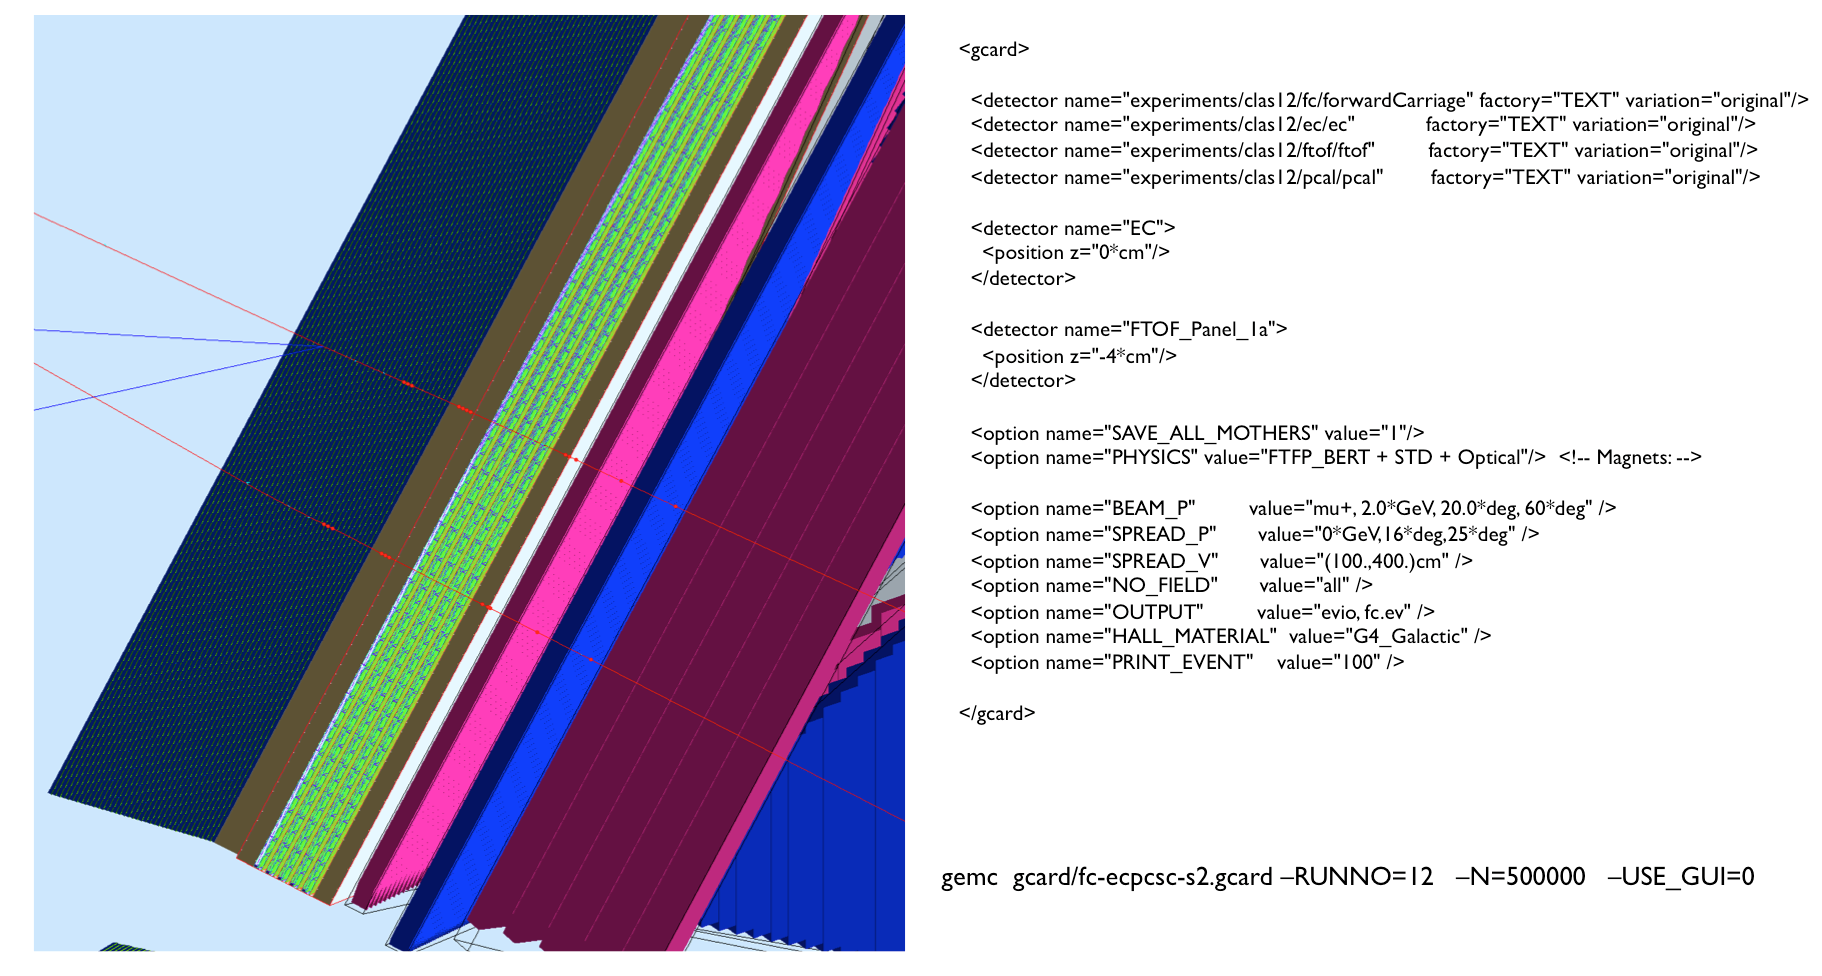
\includegraphics[width= 7in, keepaspectratio = true]{gcard}
    \caption{Snippet of the code to produce simulated events using GEMC. The graphic shows two muon tracks passing from 
    right to left.}
    \label{fig:gcard}
\end{figure}
\FloatBarrier

\subsection{Input: Generation coefficient}
The attenuation coefficients given in Tables~\ref{tab:UattenC},~\ref{tab:VattenC} and \ref{tab:WattenC} are used as the generation
coefficients. In the attenuation equation,
\begin{equation}
y = A e^{Bx} + C
\label{eq:attn}
\end{equation}
$A$, $B$ and $C$ are the attenuation coefficients and $A+C$ is defined as the gain. The gain was normalized to an \textit{ad hoc} MeV
muon. The normalized values are fed as the generation input, which, as previously mentioned, are picked up by the
\textit{gcard}. Here distance is the variable $x$.

\subsection{Cuts Applied}
Different cuts wherever relevant should be applied to ensure a more accurate calibration. The ADC distributions of the 
generated events are much cleaner as they contain no background. However, they do contain corner clippers. Therefore, to be consistent 
with the method used for the calibration of the data, two cuts are made so far: the multiplicity cut and the valid pixel cut.
These cuts are discussed below:

\subsubsection{Multiplicity Cut}
Only events with exactly one U-hit, one V-hit and one W-hit are selected. This will also help to reduce/remove events which are not
relatively perpendicular to the surface of the PCAL module. Events which do not pass this cut are removed from the analysis.

\subsubsection{Valid Pixel Cut}
Another condition required for the events to be selected is that they are within the physical shape made by the overlap. 
The database geometry provides with the coordinates of the vertices of the PCAL module which can be used to construct 
pixel and overlap shapes. Events with only one hit in these shapes in each view is only taken into account. The shapes 
which pass this cut are termed as the valid pixel/overlap shapes. Events that do not fall within these shapes are removed 
from the analysis. In other words, this cut ensures the signal track was physically valid and relatively perpendicular
with respect to the face of the PCAL module.

\FloatBarrier
\subsection{ADC signals and fits}
The events that passed the cuts are binned according to which strip is being calibrated. For example, to calibrate U-strips, bins of W
cross-strips are used. In most of these bins a Gaussian function describes the ADC distribution reasonably well. The centroids for such bins
are approximated from the Gaussian fits. However, it is also found that some bins have very small number of counts and the Gaussian
funtion can not define the distribution accurately. To account for that a fit condition is employed. If the number of events is less 
than 20, the statitical mean is used as the centroid. The process is repeated for every strip in each view. The ADC distributions and the Gaussian
fits for U67 are shown in Figures~\ref{fig:adcU1}-\ref{fig:adcU5}.
\begin{figure}[h]
    \centering
    \begin{subfigure}[h]{0.3\textwidth}
        \centering
        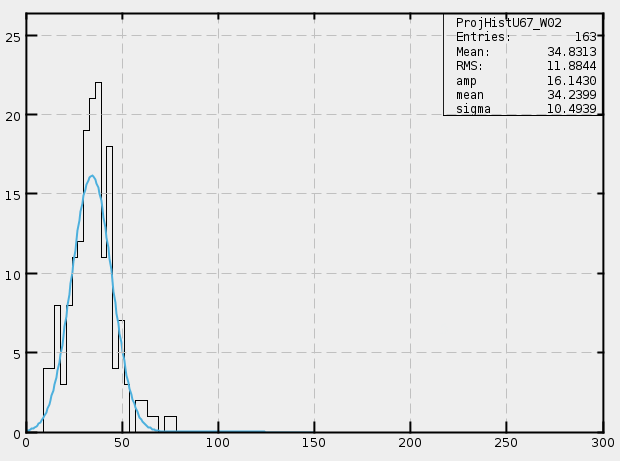
\includegraphics[width=\textwidth, keepaspectratio = true]{adcU67_02}
        \caption{adcU6702}
        \label{fig:adcU67_02}
    \end{subfigure}
    ~
    \begin{subfigure}[h]{0.3\textwidth}
        \centering
        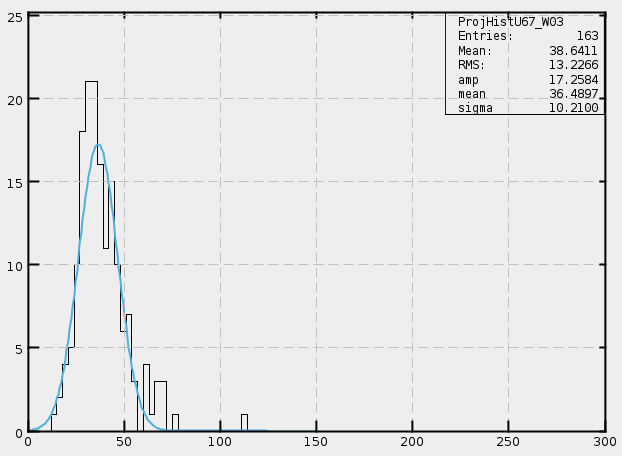
\includegraphics[width=\textwidth, keepaspectratio = true]{adcU67_03}
        \caption{adcU6703}
        \label{fig:adcU67_03}
    \end{subfigure}
    ~
    \begin{subfigure}[h]{0.3\textwidth}
        \centering
        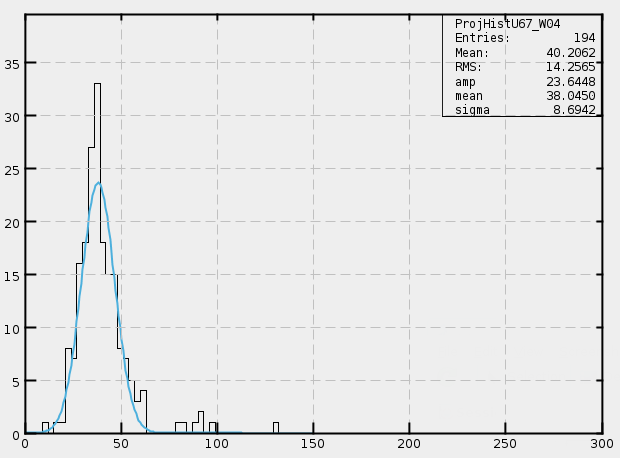
\includegraphics[width=\textwidth, keepaspectratio = true]{adcU67_04}
        \caption{adcU6704}
        \label{fig:adcU67_04}
    \end{subfigure}
    \\
    \begin{subfigure}[h]{0.3\textwidth}
        \centering
        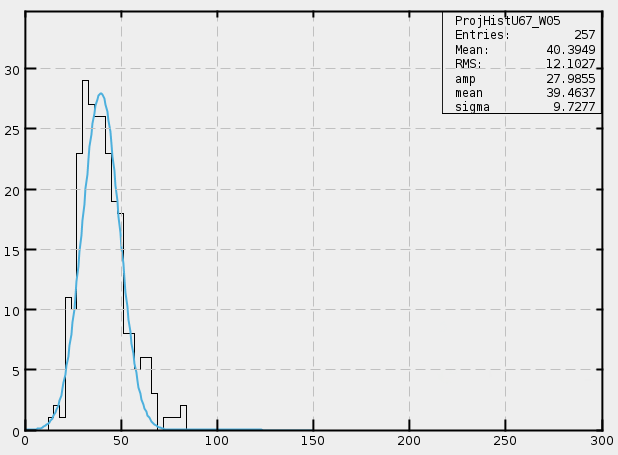
\includegraphics[width=\textwidth, keepaspectratio = true]{adcU67_05}
        \caption{adcU6705}
        \label{fig:adcU67_05}
    \end{subfigure}
    ~
    \begin{subfigure}[h]{0.3\textwidth}
        \centering
        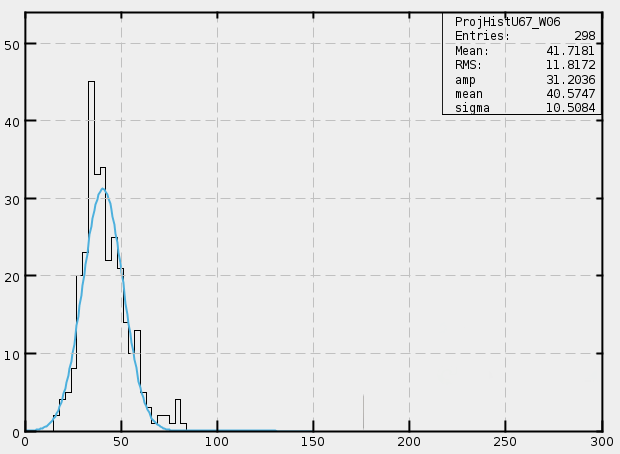
\includegraphics[width=\textwidth, keepaspectratio = true]{adcU67_06}
        \caption{adcU6706}
        \label{fig:adcU67_06}
    \end{subfigure}
    ~
    \begin{subfigure}[h]{0.3\textwidth}
        \centering
        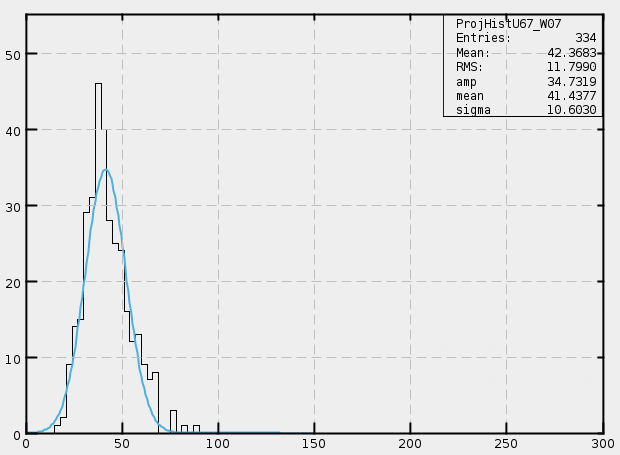
\includegraphics[width=\textwidth, keepaspectratio = true]{adcU67_07}
        \caption{adcU6707}
        \label{fig:adcU67_07}
    \end{subfigure}
    \\
    \begin{subfigure}[h]{0.3\textwidth}
        \centering
        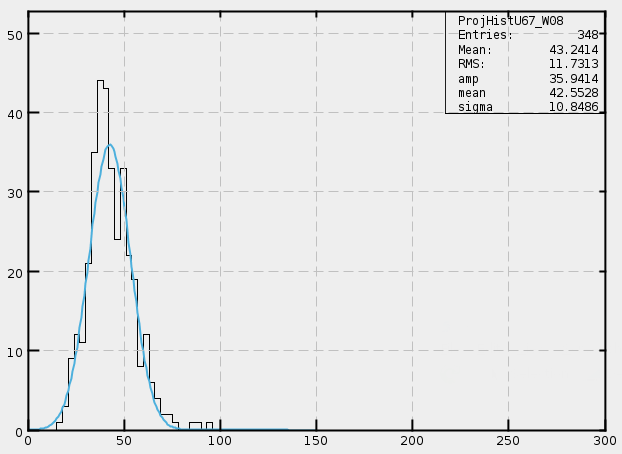
\includegraphics[width=\textwidth, keepaspectratio = true]{adcU67_08}
        \caption{adcU6708}
        \label{fig:adcU67_08}
    \end{subfigure}
    ~
    \begin{subfigure}[h]{0.3\textwidth}
        \centering
        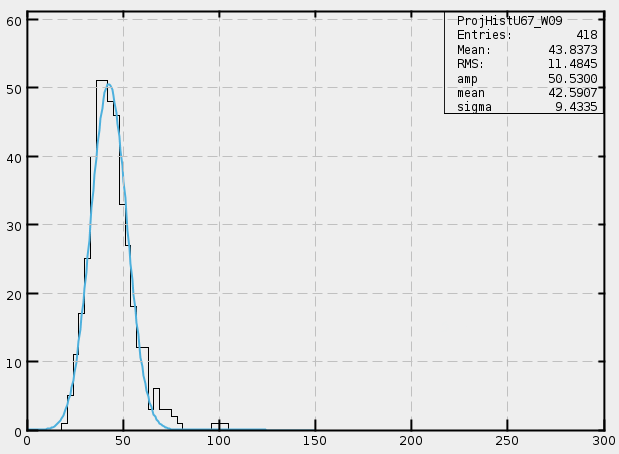
\includegraphics[width=\textwidth, keepaspectratio = true]{adcU67_09}
        \caption{adcU6709}
        \label{fig:adcU67_09}
    \end{subfigure}
    ~
    \begin{subfigure}[h]{0.3\textwidth}
        \centering
        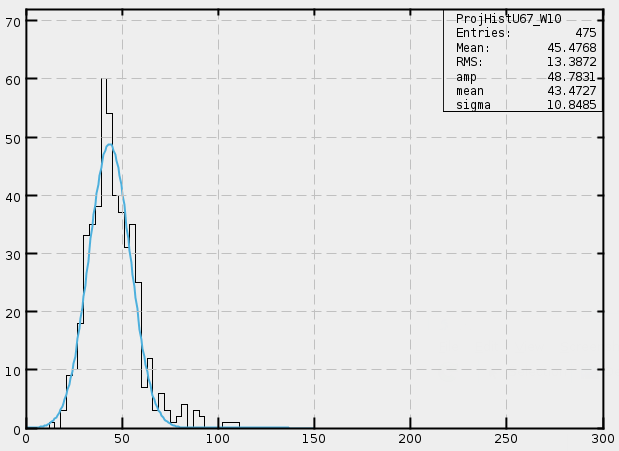
\includegraphics[width=\textwidth, keepaspectratio = true]{adcU67_10}
        \caption{adcU6710}
        \label{fig:adcU67_10}
    \end{subfigure}
    \caption{ADC distribution for U67. The last two digits in the caption of each figure represent the bin number based on the W strip.
    Blue curve is the Gaussian fit.}
    \label{fig:adcU1}
\end{figure}

\begin{figure}[h]
    \centering
    \begin{subfigure}[h]{0.3\textwidth}
        \centering
        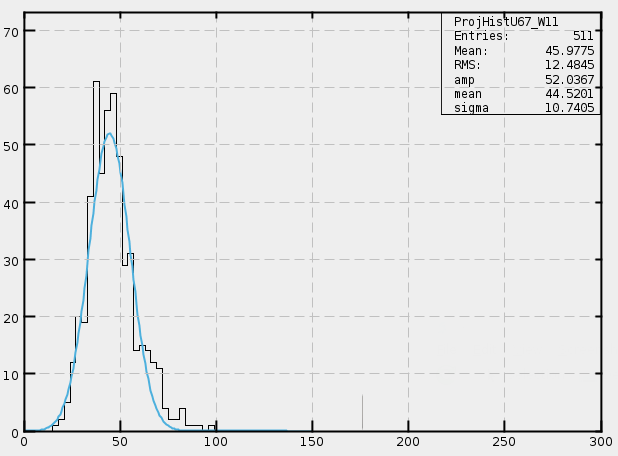
\includegraphics[width=\textwidth, keepaspectratio = true]{adcU67_11}
        \caption{adcU6711}
        \label{fig:adcU67_11}
    \end{subfigure}
    ~
    \begin{subfigure}[h]{0.3\textwidth}
        \centering
        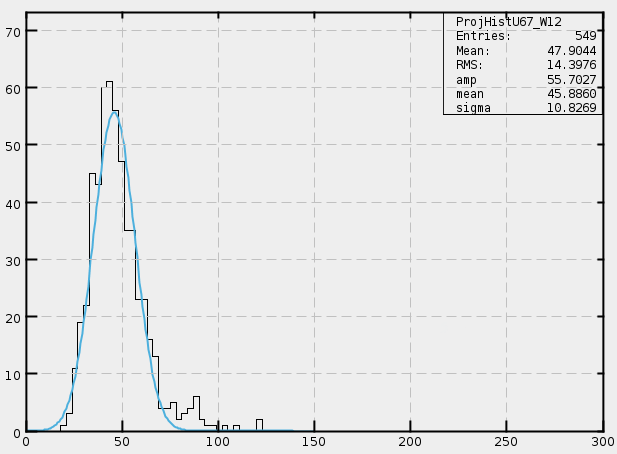
\includegraphics[width=\textwidth, keepaspectratio = true]{adcU67_12}
        \caption{adcU6712}
        \label{fig:adcU67_12}
    \end{subfigure}
    ~
    \begin{subfigure}[h]{0.3\textwidth}
        \centering
        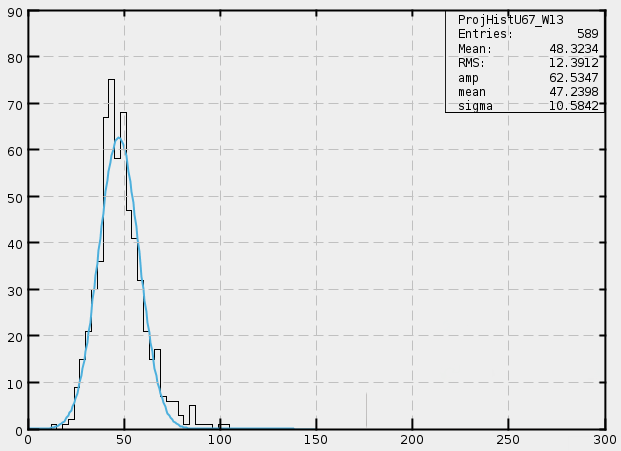
\includegraphics[width=\textwidth, keepaspectratio = true]{adcU67_13}
        \caption{adcU6713}
        \label{fig:adcU67_13}
    \end{subfigure}
    \\
    \begin{subfigure}[h]{0.3\textwidth}
        \centering
        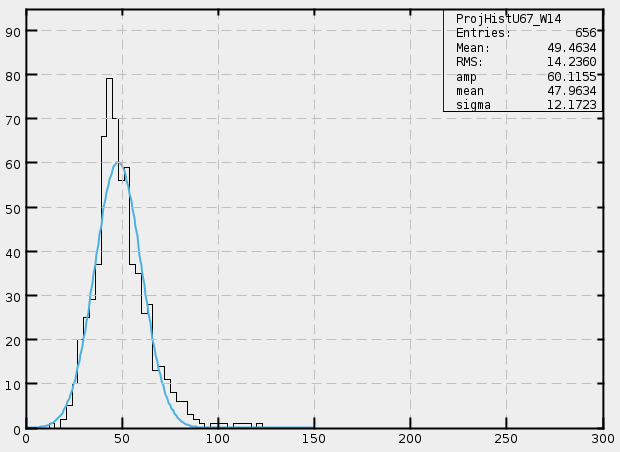
\includegraphics[width=\textwidth, keepaspectratio = true]{adcU67_14}
        \caption{adcU6714}
        \label{fig:adcU67_14}
    \end{subfigure}
    ~
    \begin{subfigure}[h]{0.3\textwidth}
        \centering
        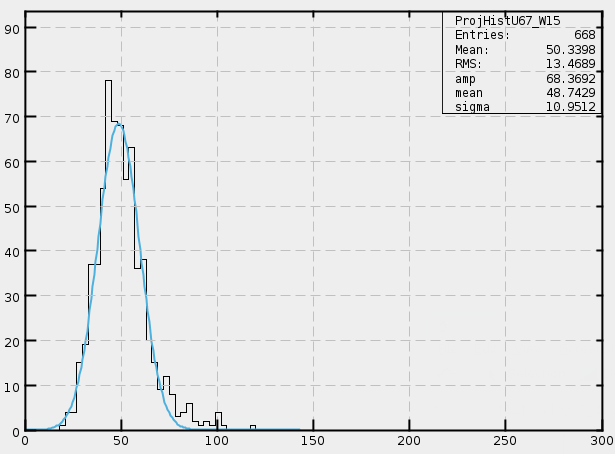
\includegraphics[width=\textwidth, keepaspectratio = true]{adcU67_15}
        \caption{adcU6715}
        \label{fig:adcU67_15}
    \end{subfigure}
    ~
    \begin{subfigure}[h]{0.3\textwidth}
        \centering
        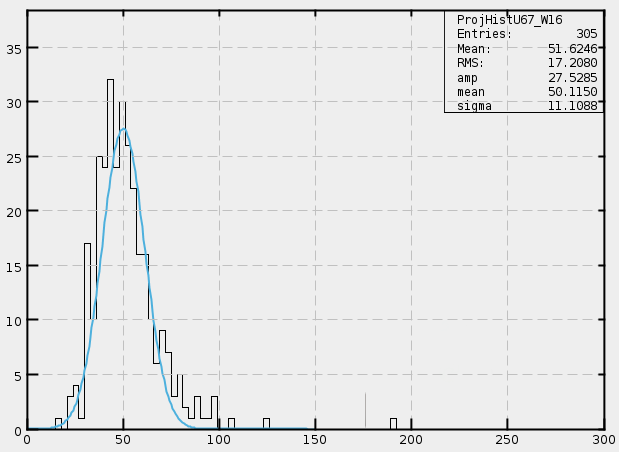
\includegraphics[width=\textwidth, keepaspectratio = true]{adcU67_16}
        \caption{adcU6716}
        \label{fig:adcU67_16}
    \end{subfigure}
    \\
    \begin{subfigure}[h]{0.3\textwidth}
        \centering
        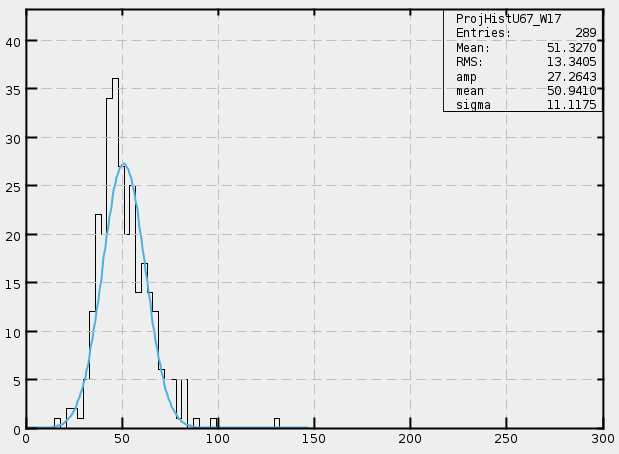
\includegraphics[width=\textwidth, keepaspectratio = true]{adcU67_17}
        \caption{adcU6717}
        \label{fig:adcU67_17}
    \end{subfigure}
    ~
    \begin{subfigure}[h]{0.3\textwidth}
        \centering
        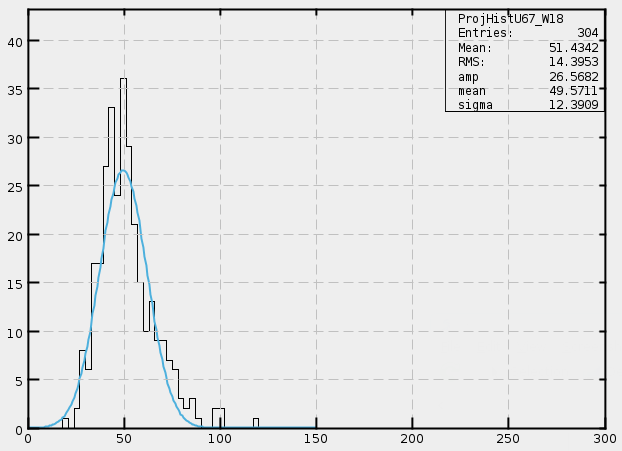
\includegraphics[width=\textwidth, keepaspectratio = true]{adcU67_18}
        \caption{adcU6718}
        \label{fig:adcU67_18}
    \end{subfigure}
    ~
    \begin{subfigure}[h]{0.3\textwidth}
        \centering
        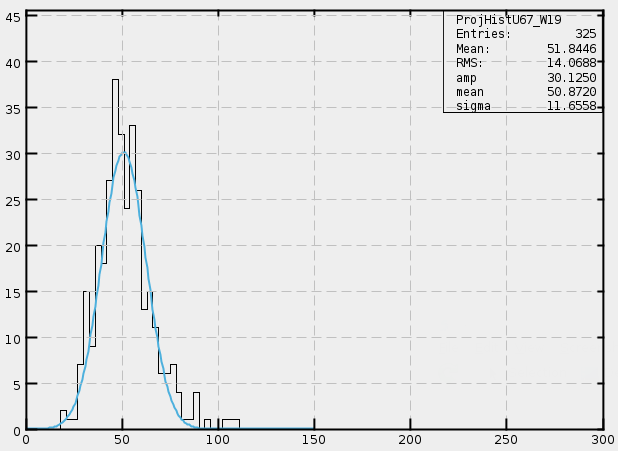
\includegraphics[width=\textwidth, keepaspectratio = true]{adcU67_19}
        \caption{adcU6718}
        \label{fig:adcU67_18}
    \end{subfigure}
    \\
    \begin{subfigure}[h]{0.3\textwidth}
        \centering
        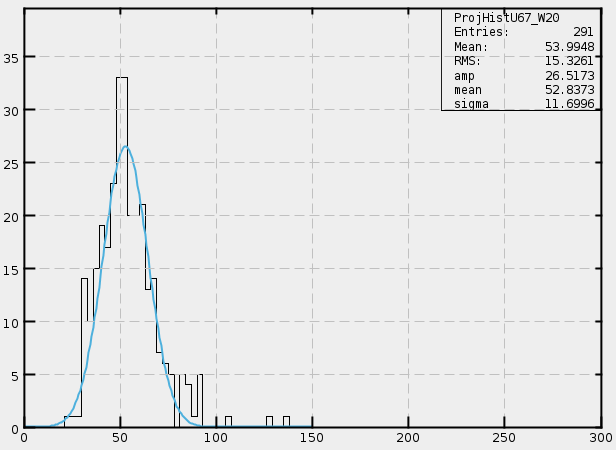
\includegraphics[width=\textwidth, keepaspectratio = true]{adcU67_20}
        \caption{adcU6720}
        \label{fig:adcU67_20}
    \end{subfigure}
    ~
    \begin{subfigure}[h]{0.3\textwidth}
        \centering
        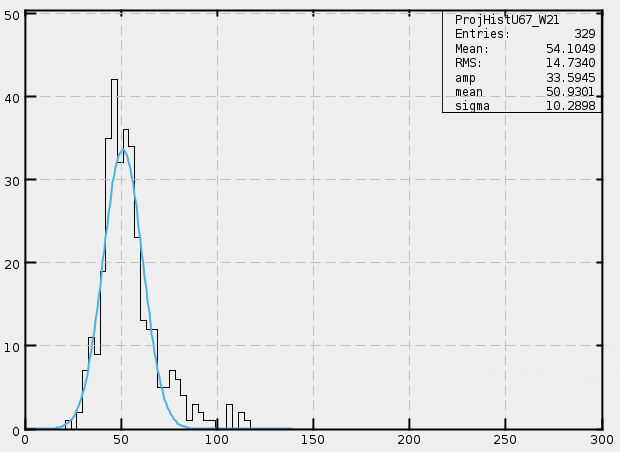
\includegraphics[width=\textwidth, keepaspectratio = true]{adcU67_21}
        \caption{adcU6721}
        \label{fig:adcU67_21}
    \end{subfigure}
    ~
    \begin{subfigure}[h]{0.3\textwidth}
        \centering
        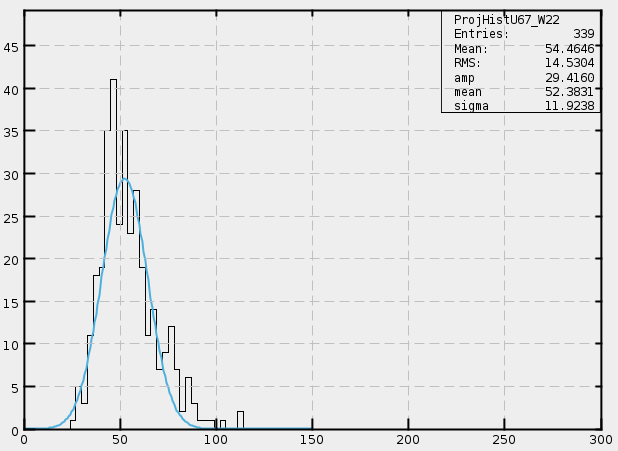
\includegraphics[width=\textwidth, keepaspectratio = true]{adcU67_22}
        \caption{adcU6722}
        \label{fig:adcU67_22}
    \end{subfigure}
    \\
    \begin{subfigure}[h]{0.3\textwidth}
        \centering
        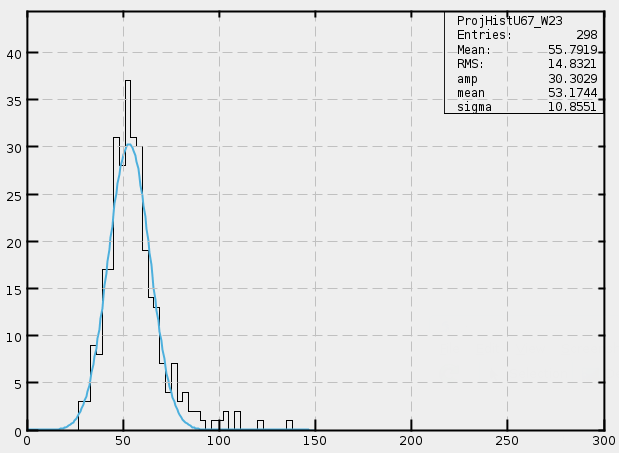
\includegraphics[width=\textwidth, keepaspectratio = true]{adcU67_23}
        \caption{adcU6723}
        \label{fig:adcU67_23}
    \end{subfigure}
    ~
    \begin{subfigure}[h]{0.3\textwidth}
        \centering
        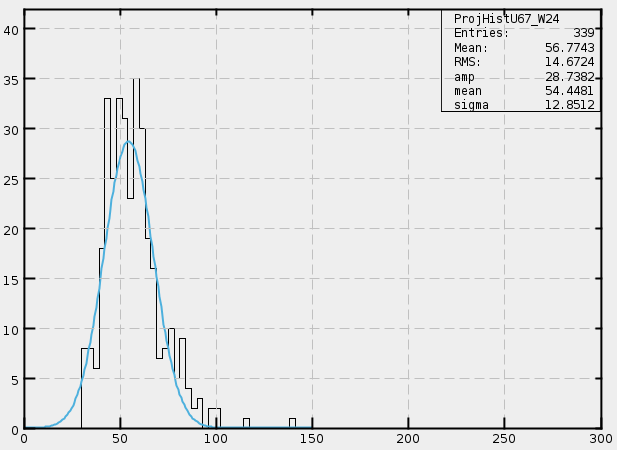
\includegraphics[width=\textwidth, keepaspectratio = true]{adcU67_24}
        \caption{adcU6724}
        \label{fig:adcU67_24}
    \end{subfigure}
    ~
    \begin{subfigure}[h]{0.3\textwidth}
        \centering
        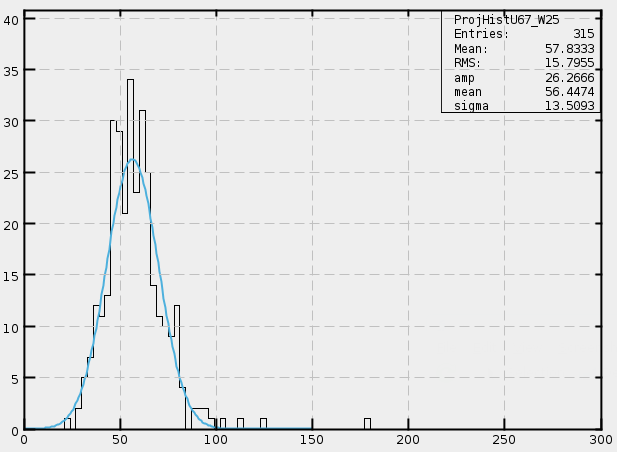
\includegraphics[width=\textwidth, keepaspectratio = true]{adcU67_25}
        \caption{adcU6725}
        \label{fig:adcU67_25}
    \end{subfigure}
    \caption{ADC distribution for U67. The last two digits in the caption of each figure represent the bin number based on the W strip.
    Blue curve is the Gaussian fit.}
    \label{fig:adcU2}
\end{figure}

\begin{figure}[h]
    \centering
    \begin{subfigure}[h]{0.3\textwidth}
        \centering
        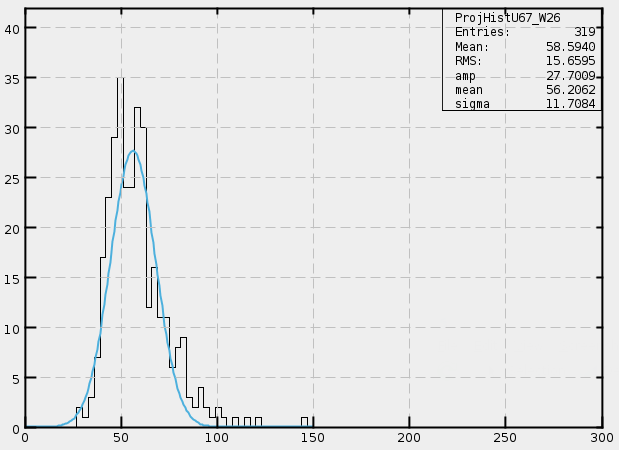
\includegraphics[width=\textwidth, keepaspectratio = true]{adcU67_26}
        \caption{adcU6726}
        \label{fig:adcU67_26}
    \end{subfigure}
    ~
    \begin{subfigure}[h]{0.3\textwidth}
        \centering
        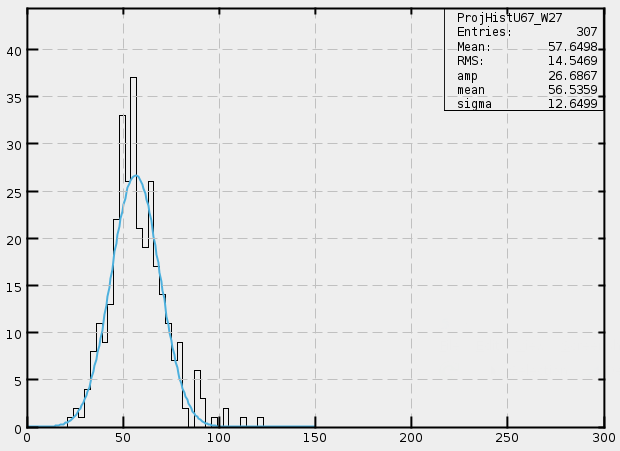
\includegraphics[width=\textwidth, keepaspectratio = true]{adcU67_27}
        \caption{adcU6727}
        \label{fig:adcU67_27}
    \end{subfigure}
    ~
    \begin{subfigure}[h]{0.3\textwidth}
        \centering
        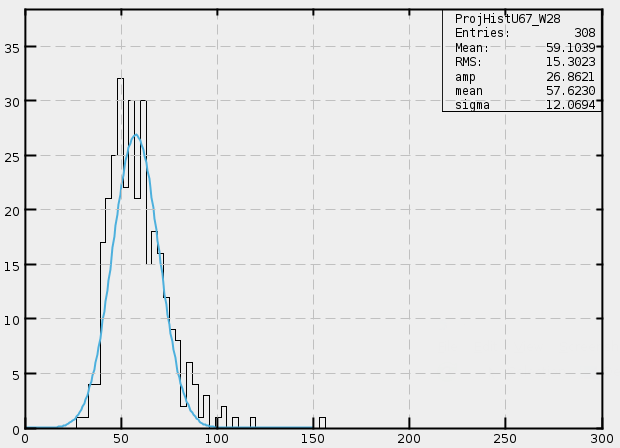
\includegraphics[width=\textwidth, keepaspectratio = true]{adcU67_28}
        \caption{adcU6728}
        \label{fig:adcU67_28}
    \end{subfigure}
    \\
    \begin{subfigure}[h]{0.3\textwidth}
        \centering
        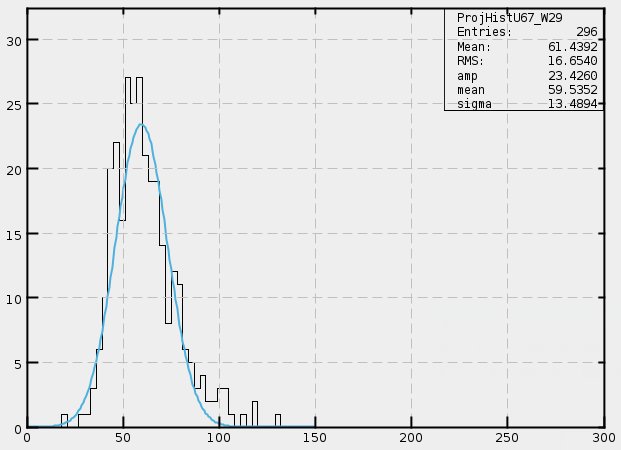
\includegraphics[width=\textwidth, keepaspectratio = true]{adcU67_29}
        \caption{adcU6729}
        \label{fig:adcU67_29}
    \end{subfigure}
    ~
    \begin{subfigure}[h]{0.3\textwidth}
        \centering
        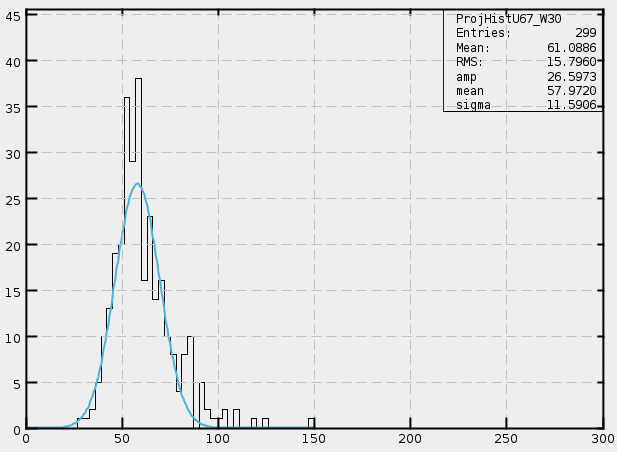
\includegraphics[width=\textwidth, keepaspectratio = true]{adcU67_30}
        \caption{adcU6730}
        \label{fig:adcU67_30}
    \end{subfigure}
    ~
    \begin{subfigure}[h]{0.3\textwidth}
        \centering
        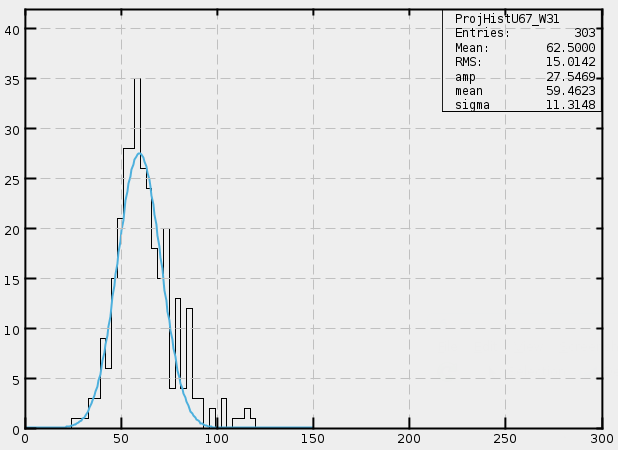
\includegraphics[width=\textwidth, keepaspectratio = true]{adcU67_31}
        \caption{adcU6731}
        \label{fig:adcU67_31}
    \end{subfigure}
    \\
    \begin{subfigure}[h]{0.3\textwidth}
        \centering
        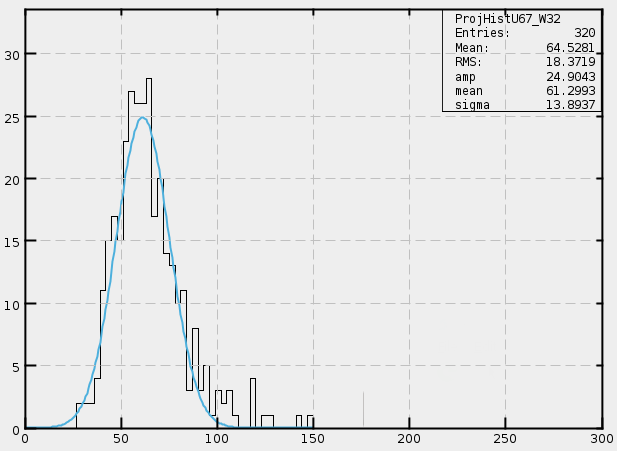
\includegraphics[width=\textwidth, keepaspectratio = true]{adcU67_32}
        \caption{adcU6732}
        \label{fig:adcU67_32}
    \end{subfigure}
    ~
    \begin{subfigure}[h]{0.3\textwidth}
        \centering
        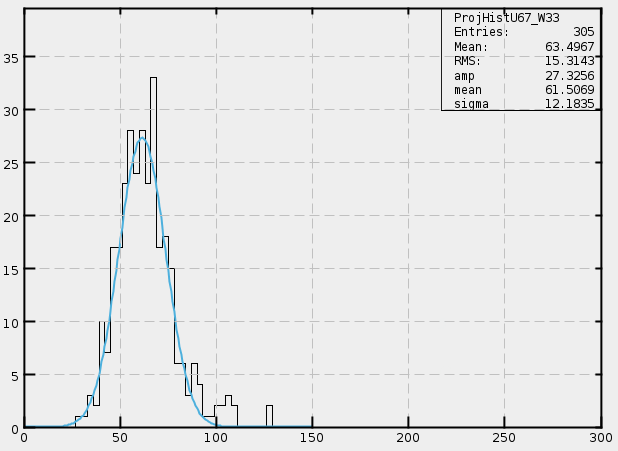
\includegraphics[width=\textwidth, keepaspectratio = true]{adcU67_33}
        \caption{adcU6733}
        \label{fig:adcU67_33}
    \end{subfigure}
    ~
    \begin{subfigure}[h]{0.3\textwidth}
        \centering
        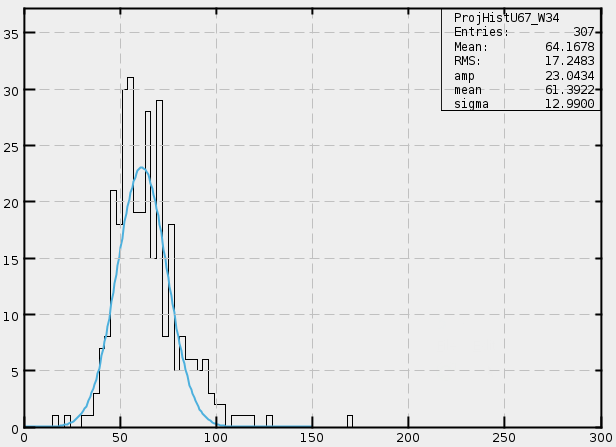
\includegraphics[width=\textwidth, keepaspectratio = true]{adcU67_34}
        \caption{adcU6734}
        \label{fig:adcU67_34}
    \end{subfigure}
    \\
    \begin{subfigure}[h]{0.3\textwidth}
        \centering
        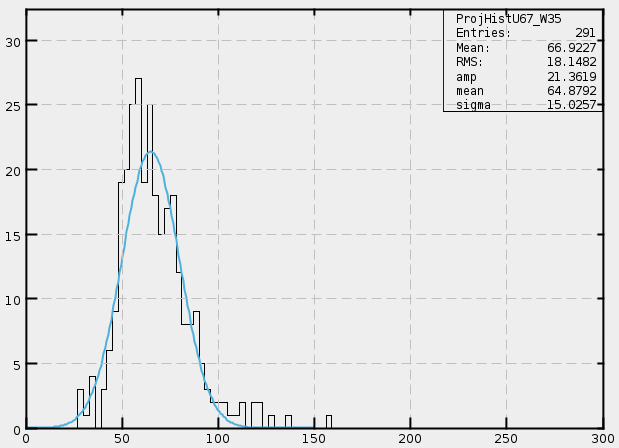
\includegraphics[width=\textwidth, keepaspectratio = true]{adcU67_35}
        \caption{adcU6735}
        \label{fig:adcU67_35}
    \end{subfigure}
    ~
    \begin{subfigure}[h]{0.3\textwidth}
        \centering
        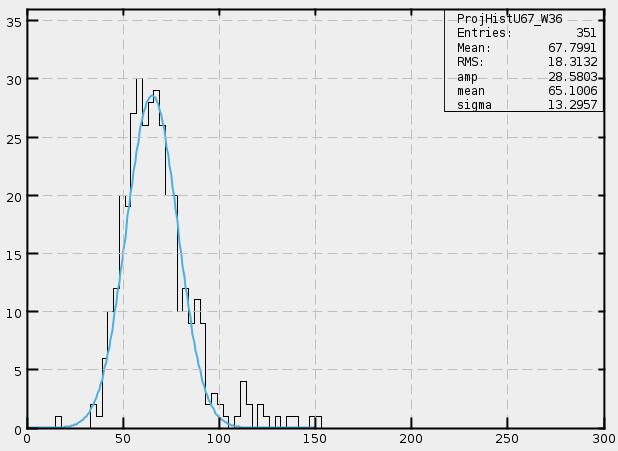
\includegraphics[width=\textwidth, keepaspectratio = true]{adcU67_36}
        \caption{adcU6736}
        \label{fig:adcU67_36}
    \end{subfigure}
    ~
    \begin{subfigure}[h]{0.3\textwidth}
        \centering
        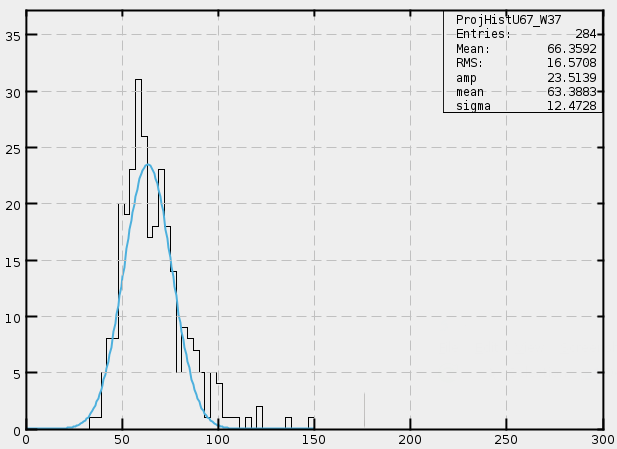
\includegraphics[width=\textwidth, keepaspectratio = true]{adcU67_37}
        \caption{adcU6737}
        \label{fig:adcU67_37}
    \end{subfigure}
    \\
    \begin{subfigure}[h]{0.3\textwidth}
        \centering
        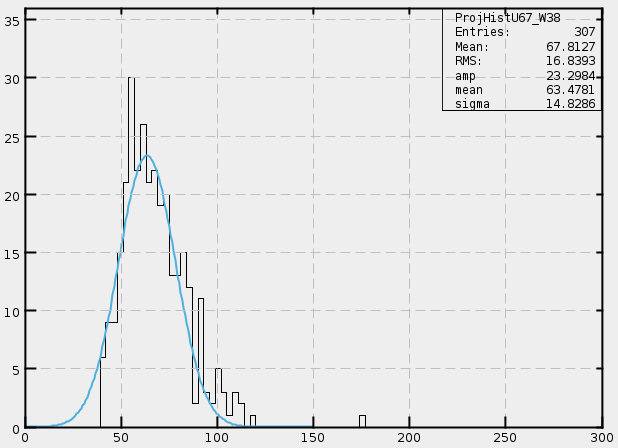
\includegraphics[width=\textwidth, keepaspectratio = true]{adcU67_38}
        \caption{adcU6738}
        \label{fig:adcU67_38}
    \end{subfigure}
    ~
    \begin{subfigure}[h]{0.3\textwidth}
        \centering
        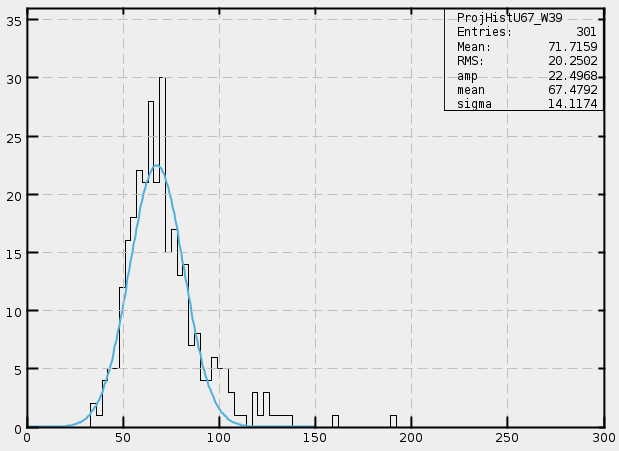
\includegraphics[width=\textwidth, keepaspectratio = true]{adcU67_39}
        \caption{adcU6739}
        \label{fig:adcU67_39}
    \end{subfigure}
    ~
    \begin{subfigure}[h]{0.3\textwidth}
        \centering
        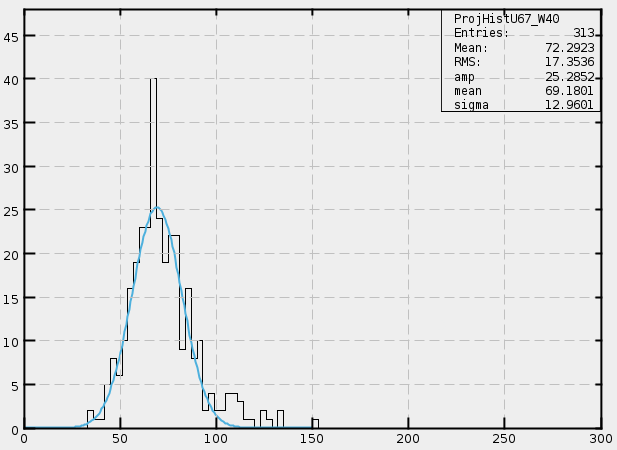
\includegraphics[width=\textwidth, keepaspectratio = true]{adcU67_40}
        \caption{adcU6740}
        \label{fig:adcU67_40}
    \end{subfigure}
    \caption{ADC distribution for U67. The last two digits in the caption of each figure represent the bin number based on the W strip.
    Blue curve is the Gaussian fit.}
    \label{fig:adcU3}
\end{figure}

\begin{figure}[h]
    \centering
    \begin{subfigure}[h]{0.3\textwidth}
        \centering
        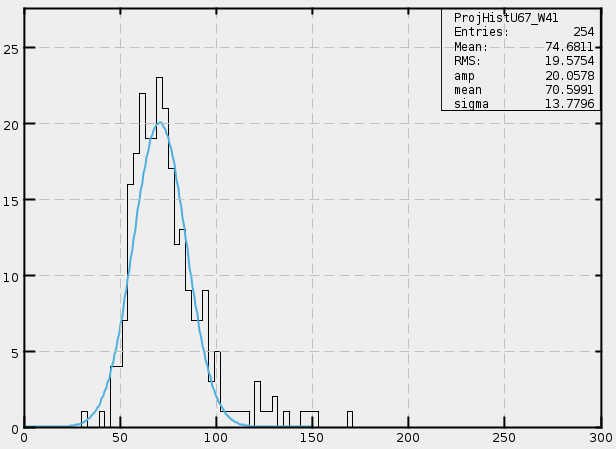
\includegraphics[width=\textwidth, keepaspectratio = true]{adcU67_41}
        \caption{adcU6741}
        \label{fig:adcU67_41}
    \end{subfigure}
    ~
    \begin{subfigure}[h]{0.3\textwidth}
        \centering
        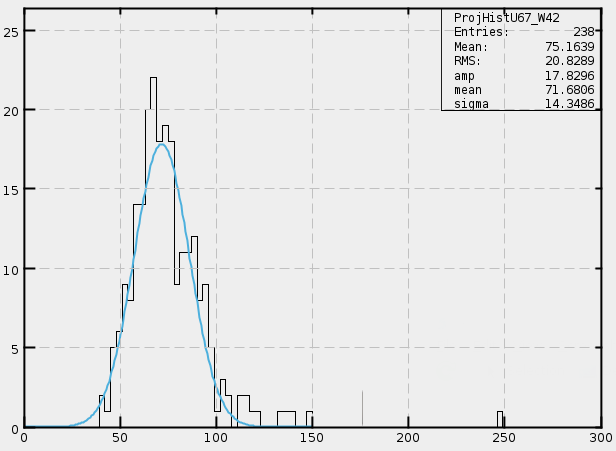
\includegraphics[width=\textwidth, keepaspectratio = true]{adcU67_42}
        \caption{adcU6742}
        \label{fig:adcU67_42}
    \end{subfigure}
    ~
    \begin{subfigure}[h]{0.3\textwidth}
        \centering
        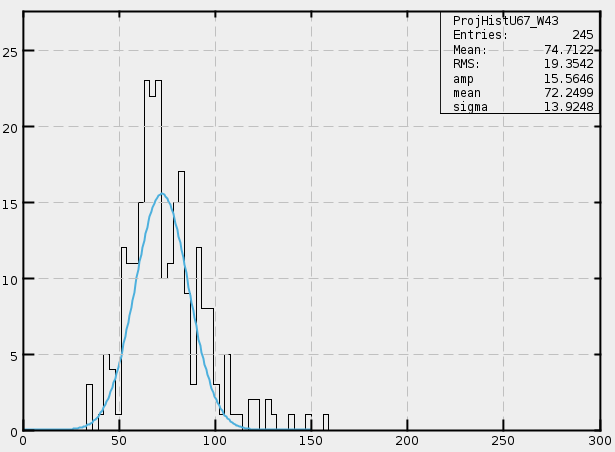
\includegraphics[width=\textwidth, keepaspectratio = true]{adcU67_43}
        \caption{adcU6743}
        \label{fig:adcU67_43}
    \end{subfigure}
    \\
    \begin{subfigure}[h]{0.3\textwidth}
        \centering
        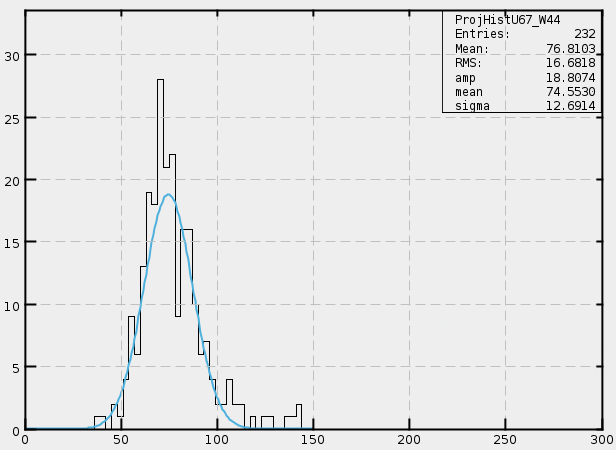
\includegraphics[width=\textwidth, keepaspectratio = true]{adcU67_44}
        \caption{adcU6744}
        \label{fig:adcU67_44}
    \end{subfigure}
    ~
    \begin{subfigure}[h]{0.3\textwidth}
        \centering
        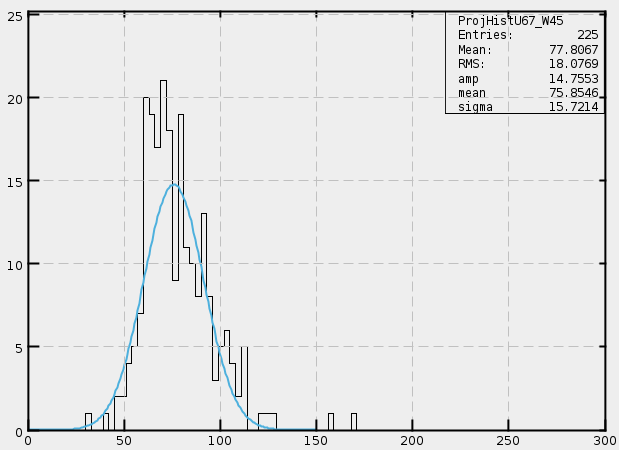
\includegraphics[width=\textwidth, keepaspectratio = true]{adcU67_45}
        \caption{adcU6745}
        \label{fig:adcU67_45}
    \end{subfigure}
    ~
    \begin{subfigure}[h]{0.3\textwidth}
        \centering
        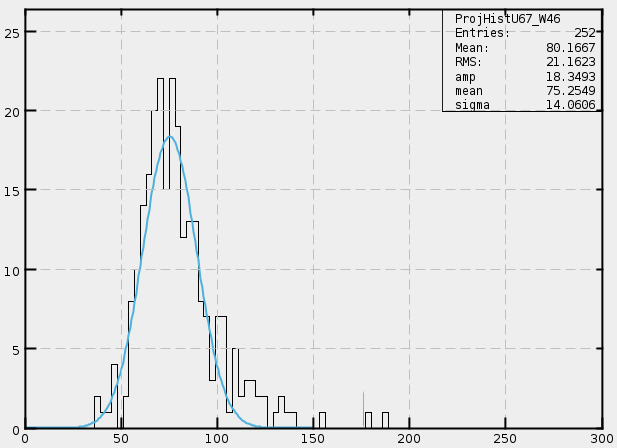
\includegraphics[width=\textwidth, keepaspectratio = true]{adcU67_46}
        \caption{adcU6746}
        \label{fig:adcU67_46}
    \end{subfigure}
    \\
    \begin{subfigure}[h]{0.3\textwidth}
        \centering
        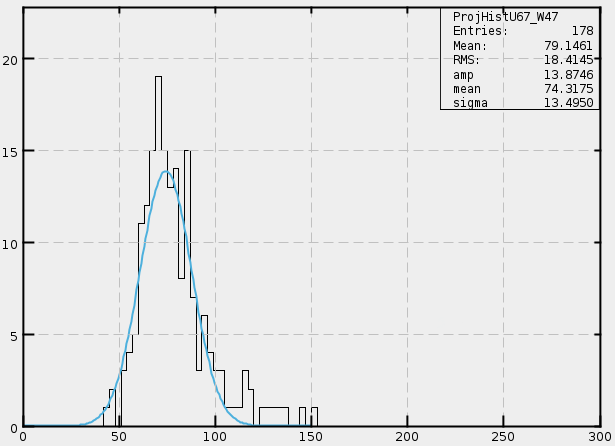
\includegraphics[width=\textwidth, keepaspectratio = true]{adcU67_47}
        \caption{adcU6747}
        \label{fig:adcU67_47}
    \end{subfigure}
    ~
    \begin{subfigure}[h]{0.3\textwidth}
        \centering
        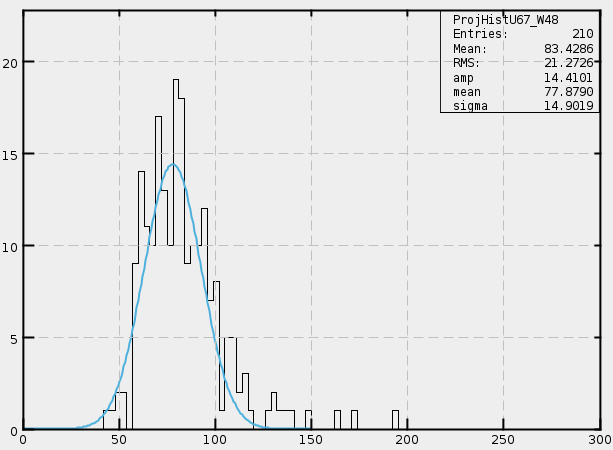
\includegraphics[width=\textwidth, keepaspectratio = true]{adcU67_48}
        \caption{adcU6748}
        \label{fig:adcU67_48}
    \end{subfigure}
    ~
    \begin{subfigure}[h]{0.3\textwidth}
        \centering
        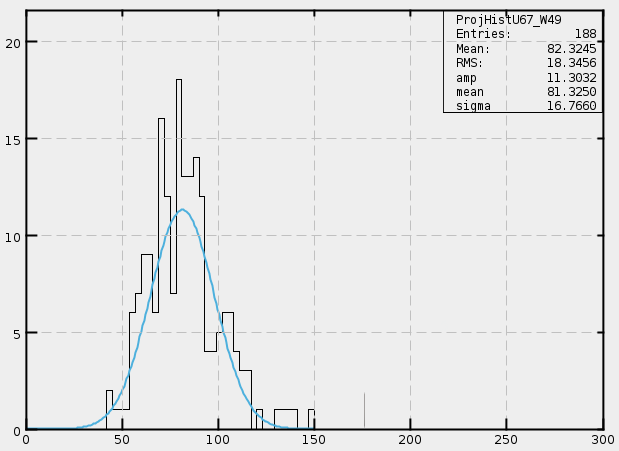
\includegraphics[width=\textwidth, keepaspectratio = true]{adcU67_49}
        \caption{adcU6749}
        \label{fig:adcU67_49}
    \end{subfigure}
    \\
    \begin{subfigure}[h]{0.3\textwidth}
        \centering
        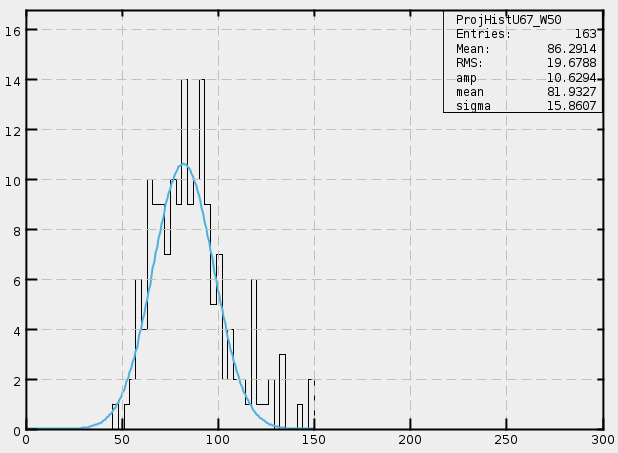
\includegraphics[width=\textwidth, keepaspectratio = true]{adcU67_50}
        \caption{adcU6750}
        \label{fig:adcU67_50}
    \end{subfigure}
    ~
    \begin{subfigure}[h]{0.3\textwidth}
        \centering
        \includegraphics[width=\textwidth, keepaspectratio = true]{adcU67_51}
        \caption{adcU6751}
        \label{fig:adcU67_51}
    \end{subfigure}
    ~
    \begin{subfigure}[h]{0.3\textwidth}
        \centering
        \includegraphics[width=\textwidth, keepaspectratio = true]{adcU67_52}
        \caption{adcU6752}
        \label{fig:adcU67_52}
    \end{subfigure}
    \\
    \begin{subfigure}[h]{0.3\textwidth}
        \centering
        \includegraphics[width=\textwidth, keepaspectratio = true]{adcU67_53}
        \caption{adcU6753}
        \label{fig:adcU67_53}
    \end{subfigure}
    ~
    \begin{subfigure}[h]{0.3\textwidth}
        \centering
        \includegraphics[width=\textwidth, keepaspectratio = true]{adcU67_54}
        \caption{adcU6754}
        \label{fig:adcU67_54}
    \end{subfigure}
    ~
    \begin{subfigure}[h]{0.3\textwidth}
        \centering
        \includegraphics[width=\textwidth, keepaspectratio = true]{adcU67_55}
        \caption{adcU6755}
        \label{fig:adcU67_55}
    \end{subfigure}
    \caption{ADC distribution for U67. The last two digits in the caption of each figure represent the bin number based on the W strip.
    Blue curve is the Gaussian fit.}
    \label{fig:adcU4}
\end{figure}

\begin{figure}[h]
    \centering
    \begin{subfigure}[h]{0.3\textwidth}
        \centering
        \includegraphics[width=\textwidth, keepaspectratio = true]{adcU67_56}
        \caption{adcU6756}
        \label{fig:adcU67_56}
    \end{subfigure}
    ~
    \begin{subfigure}[h]{0.3\textwidth}
        \centering
        \includegraphics[width=\textwidth, keepaspectratio = true]{adcU67_57}
        \caption{adcU6757}
        \label{fig:adcU67_57}
    \end{subfigure}
    ~
    \begin{subfigure}[h]{0.3\textwidth}
        \centering
        \includegraphics[width=\textwidth, keepaspectratio = true]{adcU67_58}
        \caption{adcU6758}
        \label{fig:adcU67_58}
    \end{subfigure}
    \\
    \begin{subfigure}[h]{0.3\textwidth}
        \centering
        \includegraphics[width=\textwidth, keepaspectratio = true]{adcU67_59}
        \caption{adcU6759}
        \label{fig:adcU67_59}
    \end{subfigure}
    ~
    \begin{subfigure}[h]{0.3\textwidth}
        \centering
        \includegraphics[width=\textwidth, keepaspectratio = true]{adcU67_60}
        \caption{adcU6760}
        \label{fig:adcU67_60}
    \end{subfigure}
    ~
    \begin{subfigure}[h]{0.3\textwidth}
        \centering
        \includegraphics[width=\textwidth, keepaspectratio = true]{adcU67_61}
        \caption{adcU6761}
        \label{fig:adcU67_61}
    \end{subfigure}
    \\
    \begin{subfigure}[h]{0.3\textwidth}
        \centering
        \includegraphics[width=\textwidth, keepaspectratio = true]{adcU67_62}
        \caption{adcU6762}
        \label{fig:adcU67_62}
    \end{subfigure}
    \caption{ADC distribution for U67. The last two digits in the caption of each figure represent the bin number based on the W strip.
    Blue curve is the Gaussian fit.}
    \label{fig:adcU5}
\end{figure}
\FloatBarrier
In the similar way centroids for other U-strips are extracted and stored. The correspoding distances from the center of these bins
are also evaluated. The next section deals with the exponential fits using these values to extract the calibration constants.

\FloatBarrier
\subsection{Exponential fits}
The centroid of each bin is plotted as a function of distance between the bin center to the PMT ends. An exponential funtion of the
form given in Eq.~\ref{eq:attn} is used to fit these points. The fit parameters are then extracted which are the required attenuation
 coefficients ($A$, $B$ and $C$). This process is repeated for each strip in each view so that a set of 68 U, 62 V and W coefficients 
 are recorded. To illustrate the process, the fits for ten U-strips (U51- U59 and U67) are shown in Figures~\ref{fig:expfit1}-
\ref{fig:expfit2}. As a comparison, the CCDB constants are also drawn (red curves).
\begin{figure}[h]
    \centering
    \begin{subfigure}[h]{0.44\textwidth}
        \centering
        \includegraphics[width=\textwidth, keepaspectratio = true]{expfit_U51}
        \caption{expfitU51}
        \label{fig:expfit_U51}
    \end{subfigure}
    ~
    \begin{subfigure}[h]{0.44\textwidth}
        \centering
        \includegraphics[width=\textwidth, keepaspectratio = true]{expfit_U52}
        \caption{expfitU52}
        \label{fig:expfit_U52}
    \end{subfigure}
    
    \begin{subfigure}[h]{0.44\textwidth}
        \centering
        \includegraphics[width=\textwidth, keepaspectratio = true]{expfit_U53}
        \caption{expfitU53}
        \label{fig:expfit_U53}
    \end{subfigure}
    ~
    \begin{subfigure}[h]{0.44\textwidth}
        \centering
        \includegraphics[width=\textwidth, keepaspectratio = true]{expfit_U54}
        \caption{expfitU54}
        \label{fig:expfit_U54}
    \end{subfigure}
    \caption{Exponential fits for strips U51-U54. The first set of three coeffcients are from the fit and the next set of three are
     the coefficients used in the event generation.}
    \label{fig:expfit1}
\end{figure}

\begin{figure}[h]
    \centering
    \begin{subfigure}[h]{0.44\textwidth}
        \centering
        \includegraphics[width=\textwidth, keepaspectratio = true]{expfit_U55}
        \caption{expfitU55}
        \label{fig:expfit_U55}
    \end{subfigure}
    ~
    \begin{subfigure}[h]{0.44\textwidth}
        \centering
        \includegraphics[width=\textwidth, keepaspectratio = true]{expfit_U56}
        \caption{expfitU56}
        \label{fig:expfit_U56}
    \end{subfigure}
    
    \begin{subfigure}[h]{0.44\textwidth}
        \centering
        \includegraphics[width=\textwidth, keepaspectratio = true]{expfit_U57}
        \caption{expfitU57}
        \label{fig:expfit_U57}
    \end{subfigure}
    ~
    \begin{subfigure}[h]{0.44\textwidth}
        \centering
        \includegraphics[width=\textwidth, keepaspectratio = true]{expfit_U58}
        \caption{expfitU58}
        \label{fig:expfit_U58}
    \end{subfigure}
    
    \begin{subfigure}[h]{0.44\textwidth}
        \centering
        \includegraphics[width=\textwidth, keepaspectratio = true]{expfit_U59}
        \caption{expfitU59}
        \label{fig:expfit_U59}
    \end{subfigure}
    ~
    \begin{subfigure}[h]{0.44\textwidth}
        \centering
        \includegraphics[width=\textwidth, keepaspectratio = true]{expfit_U67}
        \caption{expfitU67}
        \label{fig:expfit_U67}
    \end{subfigure}
    \caption{Exponential fits for strips U55-U59 and U67. The first set of three coeffcients are from the fit and the next set of three are
     the coefficients used in the event generation.}
    \label{fig:expfit2}
\end{figure}
\FloatBarrier

\FloatBarrier
\subsection{Attenuation Coeffiecients}
The attenuation coefficients for all the strips extracted using overlap shapes are listed in Tables~\ref{tab:UattenCSimulation},
~\ref{tab:VattenCSimulation} and ~\ref{tab:WattenCSimulation} respectively for the U, V and W views.
\begin{table}[h]
        \centering{}
        \scalebox{0.75}{
        \begin{tabular}{|c|c|c|c|}
            \hline
            U-Strip &  Parameter $A$  &Parameter $B$  & Parameter $C$ \\ \hline
1 & 51.6222 & 0 & 0 \\ \hline 
2 & 87.6722 & 0 & 0 \\ \hline 
3 & 75.2066 & 0 & 0 \\ \hline 
4 & 0 & 0 & 0 \\ \hline 
5 & 115.642 & -0.0227617 & 1.31895e-05 \\ \hline 
6 & 25.9129 & 0.0573538 & 1.84741e-11 \\ \hline 
7 & 92.8515 & -0.0111834 & 8.87529 \\ \hline 
8 & 99.9122 & -0.0071888 & 0.000272534 \\ \hline 
9 & 98.7009 & -0.00673623 & 5.30282e-05 \\ \hline 
10 & 95.7012 & -0.00501738 & 3.87816e-06 \\ \hline 
11 & 99.5796 & -0.00600944 & 5.70812e-05 \\ \hline 
12 & 101.893 & -0.0068082 & 7.35174e-05 \\ \hline 
13 & 98.5639 & -0.00536148 & 4.98004e-05 \\ \hline 
14 & 100.276 & -0.00639663 & 5.58738e-05 \\ \hline 
15 & 99.7085 & -0.00501107 & 5.66326e-05 \\ \hline 
16 & 100.059 & -0.00515426 & 5.60184e-05 \\ \hline 
17 & 98.1727 & -0.00350673 & 4.48953e-05 \\ \hline 
18 & 95.789 & -0.00272249 & 7.85182e-06 \\ \hline 
19 & 99.1342 & -0.00377288 & 5.03733e-05 \\ \hline 
20 & 100.051 & -0.00427194 & 5.98579e-05 \\ \hline 
21 & 99.1343 & -0.00399251 & 4.8361e-05 \\ \hline 
22 & 99.2099 & -0.00426886 & 4.78836e-05 \\ \hline 
23 & 99.6019 & -0.00407383 & 3.86109e-05 \\ \hline 
24 & 99.9645 & -0.00461704 & 5.33197e-05 \\ \hline 
25 & 98.7092 & -0.00440979 & 3.91902e-05 \\ \hline 
26 & 100.775 & -0.00416001 & 6.2126e-05 \\ \hline 
27 & 99.3643 & -0.00397178 & 4.43273e-05 \\ \hline 
28 & 99.8181 & -0.00397622 & 5.15282e-05 \\ \hline 
29 & 97.8789 & -0.00332809 & 2.01511e-05 \\ \hline 
30 & 99.9657 & -0.00359143 & 5.95054e-05 \\ \hline 
31 & 99.7239 & -0.00366359 & 4.3584e-05 \\ \hline 
32 & 98.0351 & -0.00356509 & 4.60719e-07 \\ \hline 
33 & 99.4801 & -0.00364831 & 4.0398e-05 \\ \hline 
34 & 99.3881 & -0.00371637 & 2.09242e-05 \\ \hline 
35 & 101.015 & -0.00372339 & 5.36132e-05 \\ \hline 
36 & 98.1016 & -0.00366948 & 0.766677 \\ \hline 
37 & 100.265 & -0.00380836 & 5.16826e-05 \\ \hline 
38 & 84.1899 & -0.00488329 & 15.3043 \\ \hline 
39 & 98.6384 & -0.00380455 & 4.01091e-07 \\ \hline 
40 & 97.8206 & -0.00349042 & 0.0308864 \\ \hline 
41 & 96.808 & -0.00352197 & 2.07162e-06 \\ \hline 
42 & 86.4983 & -0.00420312 & 11.2017 \\ \hline 
43 & 99.1538 & -0.00374538 & 1.95099e-06 \\ \hline 
44 & 98.6514 & -0.00371103 & 1.79772e-07 \\ \hline 
45 & 96.0939 & -0.00402188 & 2.2359 \\ \hline 
46 & 87.9136 & -0.00497247 & 12.1946 \\ \hline 
47 & 86.9237 & -0.00479709 & 12.3982 \\ \hline 
48 & 97.3443 & -0.00364544 & 2.5916e-07 \\ \hline 
49 & 92.823 & -0.00404197 & 6.66571 \\ \hline 
50 & 72.8505 & -0.00625032 & 24.4329 \\ \hline 
51 & 96.9279 & -0.00346737 & 7.73055e-08 \\ \hline 
52 & 95.0006 & -0.00369719 & 3.85976 \\ \hline 
53 & 83.6568 & -0.00451389 & 15.1452 \\ \hline 
54 & 70.2157 & -0.0064378 & 30.153 \\ \hline 
55 & 75.5933 & -0.00561765 & 23.3705 \\ \hline 
56 & 75.558 & -0.00589872 & 26.069 \\ \hline 
57 & 72.3298 & -0.00582056 & 25.8846 \\ \hline 
58 & 70.319 & -0.00644272 & 30.1952 \\ \hline 
59 & 73.4248 & -0.00540184 & 25.6676 \\ \hline 
60 & 75.9223 & -0.00532469 & 22.5712 \\ \hline 
61 & 90.9427 & -0.00271026 & 1.37682e-07 \\ \hline 
62 & 75.5486 & -0.00468108 & 23.8171 \\ \hline 
63 & 77.8982 & -0.00465535 & 22.7054 \\ \hline 
64 & 78.8414 & -0.00434455 & 20.5445 \\ \hline 
65 & 82.9688 & -0.0039061 & 18.0106 \\ \hline 
66 & 89.8554 & -0.00247545 & 2.51534e-08 \\ \hline 
67 & 77.6047 & -0.00440715 & 21.8361 \\ \hline 
68 & 75.2323 & -0.00463455 & 25.3975 \\ \hline  
        \end{tabular}
        }
        \caption{Calibration Constants for the U layer.}
        \label{tab:UattenCSimulation}
\end{table}

\begin{table}[h]
        \centering
        \scalebox{0.75}{
        \begin{tabular}{|c|c|c|c|}
            \hline
            V-Strip &  Parameter $A$  &Parameter $B$  & Parameter $C$ \\ \hline
1 & 81.3251 & 0 & 0 \\ \hline 
2 & 93.8447 & 0 & 0 \\ \hline 
3 & 89.258 & 0 & 0 \\ \hline 
4 & 0 & 0 & 0 \\ \hline 
5 & 112.714 & -0.0116148 & 0.000140092 \\ \hline 
6 & 108.147 & -0.00753567 & 8.66376e-09 \\ \hline 
7 & 104.461 & -0.00518872 & 2.50789e-06 \\ \hline 
8 & 45.7132 & -0.0283992 & 67.1725 \\ \hline 
9 & 99.9987 & -0.00409683 & 0.654341 \\ \hline 
10 & 103.367 & -0.00490372 & 2.64129e-07 \\ \hline 
11 & 101.999 & -0.00448106 & 8.5592e-06 \\ \hline 
12 & 101.161 & -0.00434226 & 5.51421e-06 \\ \hline 
13 & 89.4121 & -0.00480225 & 12.9398 \\ \hline 
14 & 98.3878 & -0.00325741 & 0.624151 \\ \hline 
15 & 72.3921 & -0.00538143 & 27.9022 \\ \hline 
16 & 98.7883 & -0.00352409 & 6.08974e-08 \\ \hline 
17 & 99.6729 & -0.00356374 & 3.38963e-07 \\ \hline 
18 & 100.02 & -0.0036647 & 1.82501e-07 \\ \hline 
19 & 101.396 & -0.00337965 & 3.62534e-08 \\ \hline 
20 & 89.5551 & -0.00406814 & 10.8602 \\ \hline 
21 & 100.24 & -0.00320595 & 3.83976e-07 \\ \hline 
22 & 79.997 & -0.00447596 & 21.0638 \\ \hline 
23 & 79.5925 & -0.00469138 & 21.4686 \\ \hline 
24 & 84.2625 & -0.00430666 & 16.033 \\ \hline 
25 & 87.2411 & -0.00406931 & 12.8588 \\ \hline 
26 & 99.4143 & -0.00322608 & 2.38418e-06 \\ \hline 
27 & 99.0414 & -0.00328074 & 2.68513e-08 \\ \hline 
28 & 90.6274 & -0.00369328 & 9.22529 \\ \hline 
29 & 90.2512 & -0.00396402 & 9.83799 \\ \hline 
30 & 81.0107 & -0.00490791 & 20.333 \\ \hline 
31 & 80.4556 & -0.00436419 & 18.046 \\ \hline 
32 & 95.7675 & -0.0036954 & 5.01714 \\ \hline 
33 & 86.3945 & -0.00415465 & 14.1529 \\ \hline 
34 & 81.9767 & -0.00475111 & 18.6153 \\ \hline 
35 & 86.444 & -0.00400936 & 13.1011 \\ \hline 
36 & 98.1088 & -0.00321114 & 1.63514 \\ \hline 
37 & 91.1958 & -0.00427169 & 8.74885 \\ \hline 
38 & 87.556 & -0.00374749 & 10.6152 \\ \hline 
39 & 84.6679 & -0.00480555 & 16.3922 \\ \hline 
40 & 86.1274 & -0.00410958 & 13.1448 \\ \hline 
41 & 79.803 & -0.00479862 & 21.4568 \\ \hline 
42 & 82.7876 & -0.00421391 & 17.9667 \\ \hline 
43 & 77.6727 & -0.00477563 & 24.3102 \\ \hline 
44 & 82.7088 & -0.00433188 & 17.2481 \\ \hline 
45 & 81.0337 & -0.00505961 & 20.0948 \\ \hline 
46 & 83.7595 & -0.00407532 & 14.8532 \\ \hline 
47 & 81.9191 & -0.00453048 & 18.6102 \\ \hline 
48 & 86.6122 & -0.00409001 & 14.6335 \\ \hline 
49 & 84.7559 & -0.00461439 & 16.8 \\ \hline 
50 & 84.9907 & -0.00415237 & 16.3736 \\ \hline 
51 & 82.6795 & -0.00486204 & 18.6174 \\ \hline 
52 & 85.7642 & -0.00455222 & 15.118 \\ \hline 
53 & 85.23 & -0.00445134 & 15.377 \\ \hline 
54 & 84.2234 & -0.00451731 & 17.081 \\ \hline 
55 & 83.6998 & -0.00428485 & 16.7591 \\ \hline 
56 & 84.6766 & -0.00440632 & 14.549 \\ \hline 
57 & 84.574 & -0.00386128 & 15.0527 \\ \hline 
58 & 86.9262 & -0.00392846 & 12.2401 \\ \hline 
59 & 82.764 & -0.00404404 & 15.0655 \\ \hline 
60 & 85.8456 & -0.00382857 & 12.7791 \\ \hline 
61 & 84.1674 & -0.00396819 & 15.3756 \\ \hline 
62 & 77.0637 & -0.00309805 & 8.36148 \\ \hline 
        \end{tabular}
        }
        \caption{Calibration Constants for the V layer.}
        \label{tab:VattenCSimulation}
\end{table}

\begin{table}[h]
        \centering
        \scalebox{0.75}{
        \begin{tabular}{|c|c|c|c|}
            \hline
            W-Strip &  Parameter $A$  &Parameter $B$  & Parameter $C$ \\ \hline
1 & 76.5834 & 0 & 0 \\ \hline 
2 & 94.6674 & 0 & 0 \\ \hline 
3 & 0 & 0 & 0 \\ \hline 
4 & 109.142 & -0.0130086 & 0.00015922 \\ \hline 
5 & 107.035 & -0.00894442 & 8.24225e-07 \\ \hline 
6 & 105.492 & -0.00708408 & 1.33493e-05 \\ \hline 
7 & 96.1992 & -0.00724769 & 11.9308 \\ \hline 
8 & 98.279 & -0.00491833 & 1.82152 \\ \hline 
9 & 49.0971 & -0.0127096 & 55.5526 \\ \hline 
10 & 94.9267 & -0.00399965 & 5.86104 \\ \hline 
11 & 102.166 & -0.00463505 & 7.03285e-06 \\ \hline 
12 & 102.1 & -0.00427262 & 1.17733e-06 \\ \hline 
13 & 88.889 & -0.00478508 & 12.4618 \\ \hline 
14 & 95.8496 & -0.00374209 & 5.45295 \\ \hline 
15 & 77.3844 & -0.00529214 & 25.067 \\ \hline 
16 & 100.583 & -0.00404282 & 2.15117e-07 \\ \hline 
17 & 96.9804 & -0.0038156 & 1.44707e-05 \\ \hline 
18 & 99.9379 & -0.00396405 & 2.17298e-05 \\ \hline 
19 & 75.9695 & -0.00514872 & 21.2028 \\ \hline 
20 & 71.233 & -0.00617771 & 28.0456 \\ \hline 
21 & 77.7536 & -0.00547851 & 23.1228 \\ \hline 
22 & 99.7207 & -0.00369463 & 1.71972e-05 \\ \hline 
23 & 98.6427 & -0.00343161 & 1.23854e-06 \\ \hline 
24 & 100.039 & -0.00387015 & 3.2979e-06 \\ \hline 
25 & 82.408 & -0.00501709 & 16.3269 \\ \hline 
26 & 99.6441 & -0.00372218 & 1.05835e-07 \\ \hline 
27 & 93.5772 & -0.00365972 & 5.49534 \\ \hline 
28 & 91.8945 & -0.00409323 & 8.37447 \\ \hline 
29 & 86.8697 & -0.00452968 & 14.2807 \\ \hline 
30 & 84.8415 & -0.00458064 & 15.0535 \\ \hline 
31 & 79.2046 & -0.00520979 & 22.875 \\ \hline 
32 & 77.2896 & -0.00508816 & 23.2359 \\ \hline 
33 & 82.1087 & -0.00533502 & 19.7361 \\ \hline 
34 & 89.4605 & -0.00406 & 10.7605 \\ \hline 
35 & 88.6131 & -0.00375663 & 10.4811 \\ \hline 
36 & 97.2606 & -0.0033744 & 2.02937 \\ \hline 
37 & 86.0419 & -0.00461505 & 14.1821 \\ \hline 
38 & 83.2823 & -0.00477393 & 18.1849 \\ \hline 
39 & 80.9365 & -0.00487184 & 19.3808 \\ \hline 
40 & 86.8735 & -0.00415256 & 13.2762 \\ \hline 
41 & 86.8237 & -0.00428351 & 14.3152 \\ \hline 
42 & 87.9619 & -0.00388999 & 11.4198 \\ \hline 
43 & 83.4599 & -0.00446605 & 16.7767 \\ \hline 
44 & 84.7084 & -0.00409597 & 14.6483 \\ \hline 
45 & 85.7983 & -0.00418715 & 14.7523 \\ \hline 
46 & 78.5469 & -0.0046913 & 22.0838 \\ \hline 
47 & 80.8861 & -0.00455342 & 19.7712 \\ \hline 
48 & 85.9249 & -0.00390414 & 14.0986 \\ \hline 
49 & 84.238 & -0.00427813 & 14.5056 \\ \hline 
50 & 80.7529 & -0.00426804 & 18.3437 \\ \hline 
51 & 81.6971 & -0.00434176 & 16.7262 \\ \hline 
52 & 73.9153 & -0.00529965 & 27.8944 \\ \hline 
53 & 83.048 & -0.00254593 & 7.55929e-09 \\ \hline 
54 & 81.2306 & -0.00447303 & 18.2888 \\ \hline 
55 & 85.9745 & -0.00421353 & 12.3989 \\ \hline 
56 & 80.6208 & -0.00523589 & 22.6337 \\ \hline 
57 & 87.486 & -0.00368434 & 9.59789 \\ \hline 
58 & 81.3392 & -0.00504944 & 21.1264 \\ \hline 
59 & 86.0705 & -0.00417194 & 12.3202 \\ \hline 
60 & 84.3917 & -0.00441815 & 14.8435 \\ \hline 
61 & 77.2549 & -0.0049831 & 23.2266 \\ \hline 
62 & 78.4089 & -0.00232346 & 8.83974e-07 \\ \hline  
        \end{tabular}
        }
        \caption{Calibration Constants for the W layer.}
        \label{tab:WattenCSimulation}
\end{table}
\FloatBarrier
